\section{Resultados e discussão dos resultados}\label{sec:resultados}

Esta seção apresenta os resultados obtidos nos experimentos de verificação biométrica com os modelos DeepPrint e FLARE (e suas respectivas variações de alinhamento e realce) sobre as partições de avaliação principal (Parte A) dos sensores reais (DB1 a DB3) das edições FVC2000, FVC2002 e FVC2004, e os resultados do MCC com a parte FVC2000, bem como sobre os conjuntos de dados CrossMatch e U.are.U disponibilizados pela Neurotechnology.

A Tabela~\ref{tab:eer_base} apresenta a comparação de EER obtida pelas abordagens base (sem realce) no ponto de mínima diferença entre FAR e FRR. O método MCC foi avaliado nas bases da edição FVC2000 e da Neurotechnology. Foram também realizados experimentos para avaliar o efeito do realce (PriorEnh e UNetEnh) sobre o desempenho dos modelos. Entretanto, no geral, o realce não aprimorou o desempenho. O resultado dessa avaliação adicional está disponível no repositório no Github\footnote{\url{https://github.com/Thiago-Fernandes-Dias/ic_2025_experimentos}} com o código-fonte dos experimentos.

\begin{table}[htbp]
\centering
\small
\caption{EER (\%) dos métodos base (sem realce) nos subconjuntos Parte A do FVC e nas bases da Neurotechnology.}\label{tab:eer_base}
\setlength{\tabcolsep}{7pt}
\begin{tabular}{ll rrrr}
\toprule
\textbf{Edição / Origem} & \textbf{Base} & \textbf{DeepPrint} & \textbf{FLARE (Reg.)} & \textbf{FLARE (Vot.)} & \textbf{MCC} \\
\midrule
FVC2000 & DB1-A & 3.36 & 0.81 & 0.81 & 2.69 \\
 & DB2-A & 2.69 & 0.54 & 0.19 & 4.33 \\
 & DB3-A & 3.85 & 0.63 & 0.59 & 10.21 \\
\cmidrule{2-6}
\multicolumn{2}{l}{\textbf{Média FVC2000}} & \textbf{3.30} & \textbf{0.66} & \textbf{0.53} & \textbf{5.74} \\
\midrule
FVC2002 & DB1-A & 5.20 & 0.44 & 0.25 & -- \\
 & DB2-A & 8.19 & 0.62 & 0.69 & -- \\
 & DB3-A & 8.51 & 3.32 & 2.08 & -- \\
\cmidrule{2-6}
\multicolumn{2}{l}{\textbf{Média FVC2002}} & \textbf{7.30} & \textbf{1.46} & \textbf{1.01} & -- \\
\midrule
FVC2004 & DB1-A & 17.05 & 0.25 & 0.24 & -- \\
 & DB2-A & 5.27 & 1.44 & 0.87 & -- \\
 & DB3-A & 4.91 & 0.38 & 0.31 & -- \\
\cmidrule{2-6}
\multicolumn{2}{l}{\textbf{Média FVC2004}} & \textbf{9.08} & \textbf{0.69} & \textbf{0.47} & -- \\
\midrule
\multicolumn{2}{l}{\textbf{Média FVC}} & \textbf{6.56} & \textbf{0.94} & \textbf{0.67} & -- \\
\midrule
Neurotechnology & CrossMatch & 3.31 & 0.49 & 0.12 & 2.10 \\
 & U.are.U & 2.76 & 0.58 & 0.86 & 1.94 \\
\cmidrule{2-6}
\multicolumn{2}{l}{\textbf{Média Neurotechnology}} & \textbf{3.04} & \textbf{0.53} & \textbf{0.49} & \textbf{2.02} \\
\midrule[\heavyrulewidth]
\multicolumn{2}{l}{\textbf{Média Geral}} & \textbf{5.92} & \textbf{0.86} & \textbf{0.64} & -- \\
\bottomrule
\end{tabular}
\end{table}

A Figura~\ref{fig:histograms_fvc2000} apresenta a comparação da distribuição das pontuações de similaridade entre DeepPrint, FLARE (com alinhamento por votação) e MCC para o subconjunto DB1-A da edição FVC2000. Observa-se que, no FLARE, a distribuição das pontuações de impostores (vermelho) permanece concentrada em valores baixos (próximos a 0,2), resultando em uma separação quase total em relação aos usuários genuínos (verde) e justificando as taxas de EER substancialmente menores em comparação ao DeepPrint e ao MCC. No MCC, a sobreposição entre as distribuições no DB1-A é ligeiramente inferior à do DeepPrint, refletindo a menor EER (2,69\% contra 3,36\%). Os histogramas para os demais conjuntos de dados estão disponíveis no repositório no GitHub e apresentam tendências similares às observadas nos histogramas destacados.

\begin{figure}[htbp]
\centering
\subfloat[DeepPrint - DB1-A]{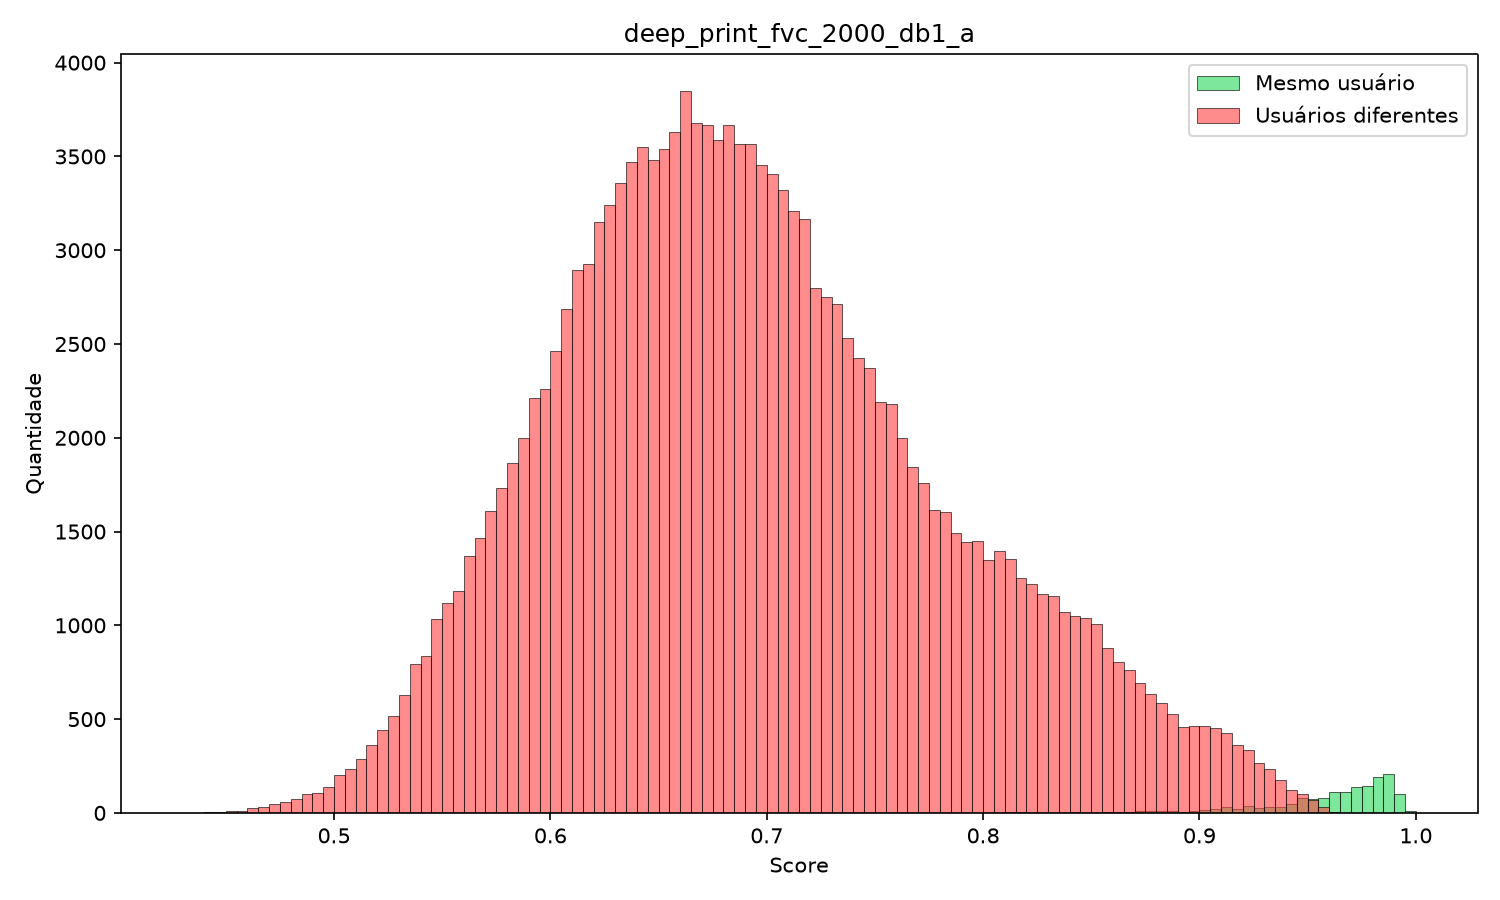
\includegraphics[width=0.32\textwidth]{figures/histograms/deep_print_fvc_2000_db1_a.png}}
\hfill
\subfloat[FLARE (Votação) - DB1-A]{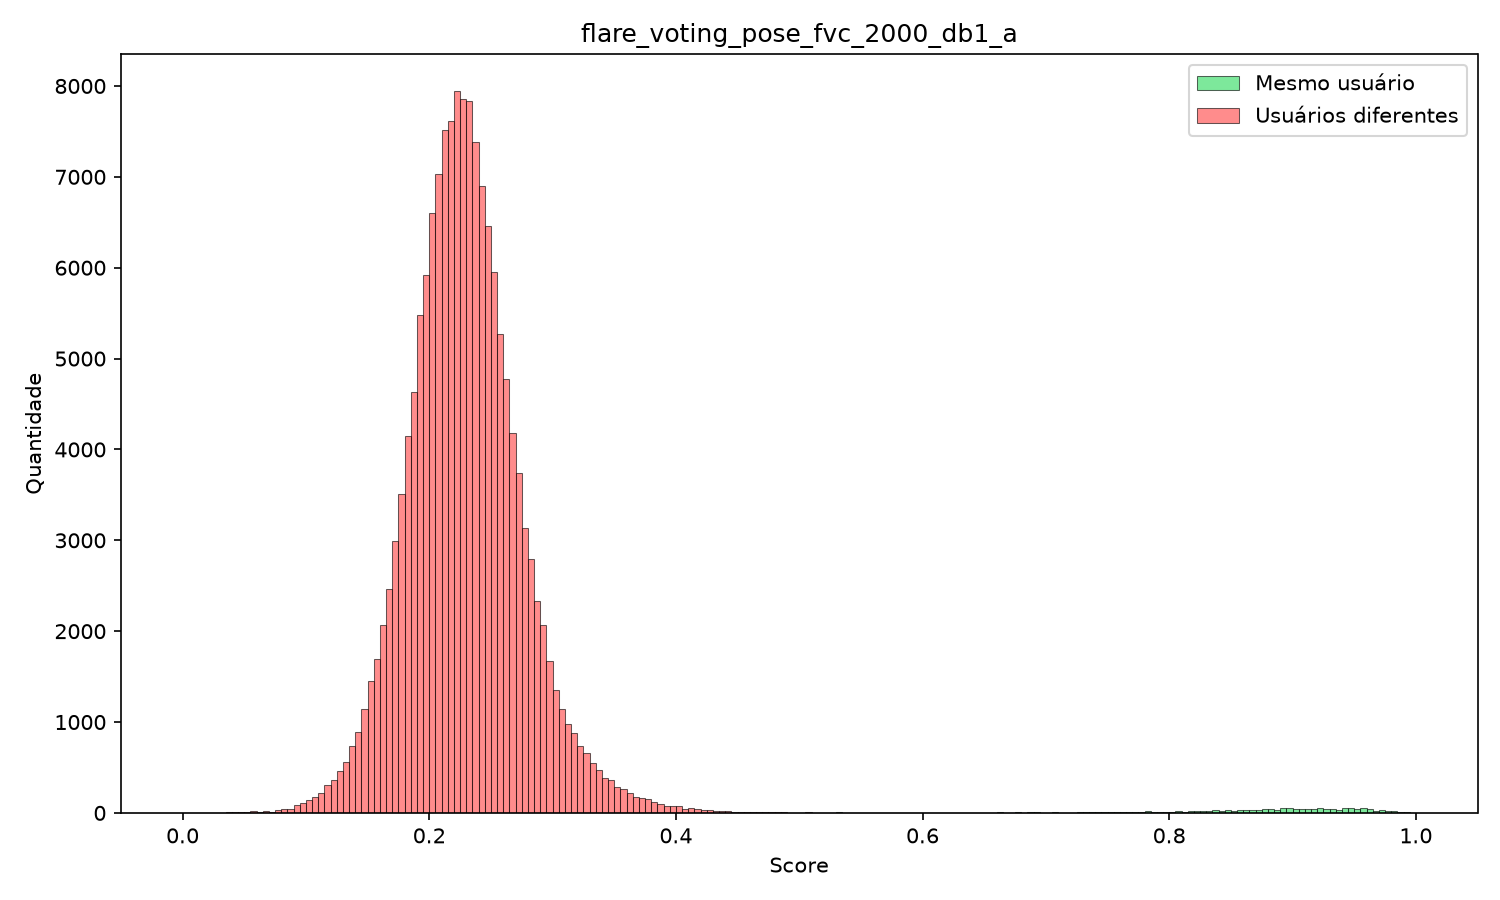
\includegraphics[width=0.32\textwidth]{figures/histograms/flare_voting_pose_fvc_2000_db1_a.png}}
\hfill
\subfloat[MCC - DB1-A]{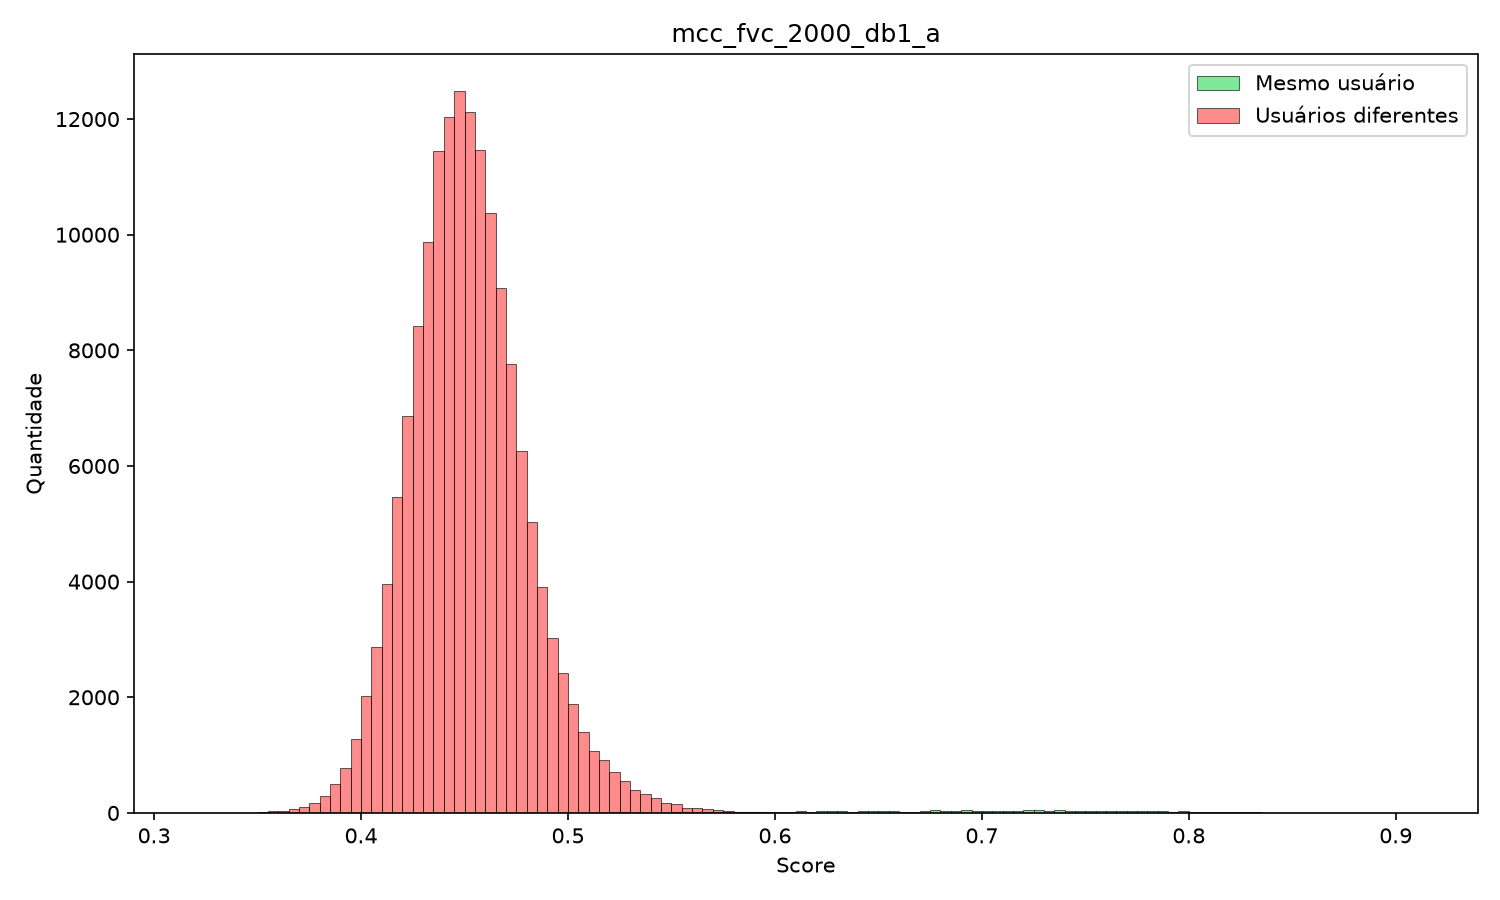
\includegraphics[width=0.32\textwidth]{figures/histograms/mcc_fvc_2000_db1_a.png}}

\caption{Comparação da distribuição das pontuações de similaridade entre DeepPrint, FLARE com alinhamento por votação e MCC para o subconjunto DB1-A do FVC2000.}\label{fig:histograms_fvc2000}
\end{figure}

A Figura~\ref{fig:histograms_neurotechnology} apresenta a comparação das pontuações entre o DeepPrint, o FLARE (alinhamento por votação) e o MCC para os conjuntos CrossMatch e U.are.U da Neurotechnology. Nessas bases, capturadas por sensores ópticos de alta qualidade, o MCC apresenta separação superior à do DeepPrint (EER de 2,10\% no CrossMatch e 1,94\% no U.are.U, frente a 3,31\% e 2,76\% do DeepPrint), enquanto o FLARE mantém o melhor poder discriminativo geral (EER de 0,12\% e 0,86\%, respectivamente).

\begin{figure}[htbp]
\centering
\subfloat[DeepPrint - CrossMatch]{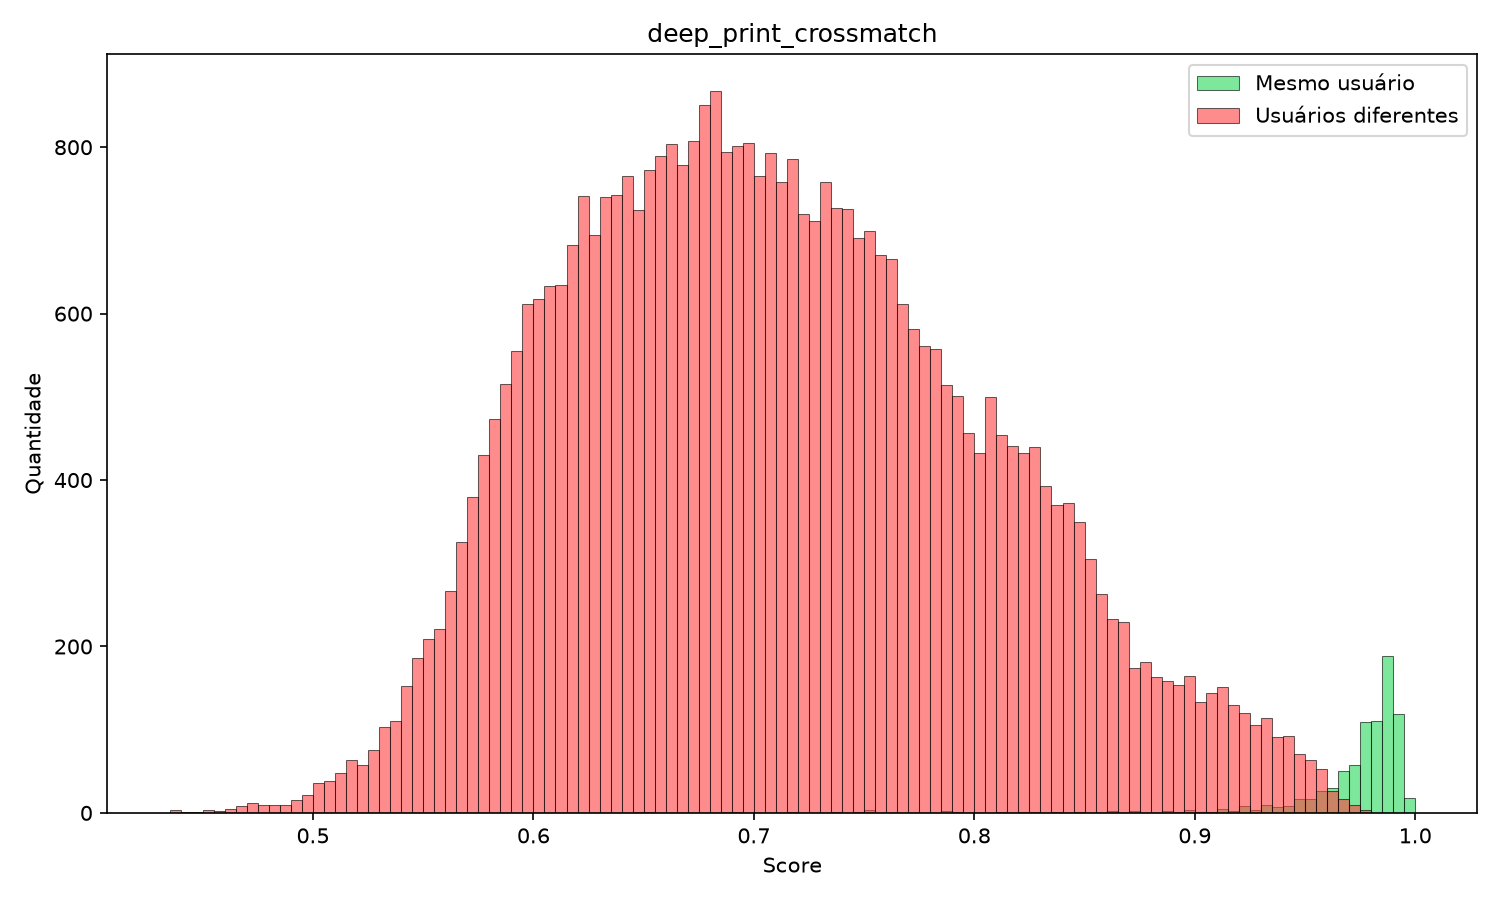
\includegraphics[width=0.32\textwidth]{figures/histograms/deep_print_crossmatch.png}}
\hfill
\subfloat[FLARE (Votação) - CrossMatch]{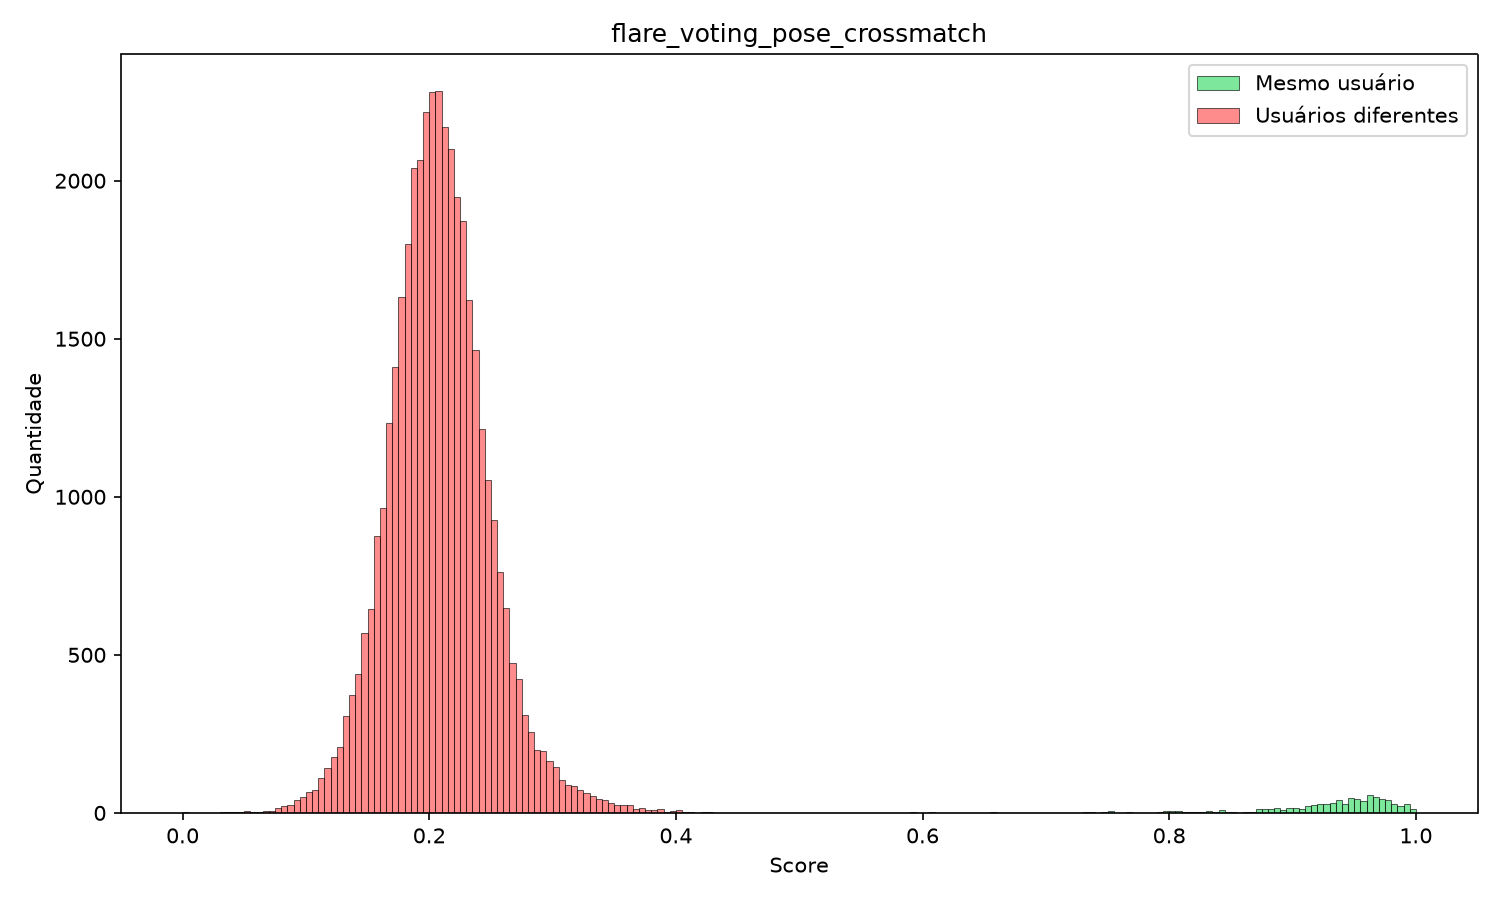
\includegraphics[width=0.32\textwidth]{figures/histograms/flare_voting_pose_crossmatch.png}}
\hfill
\subfloat[MCC - CrossMatch]{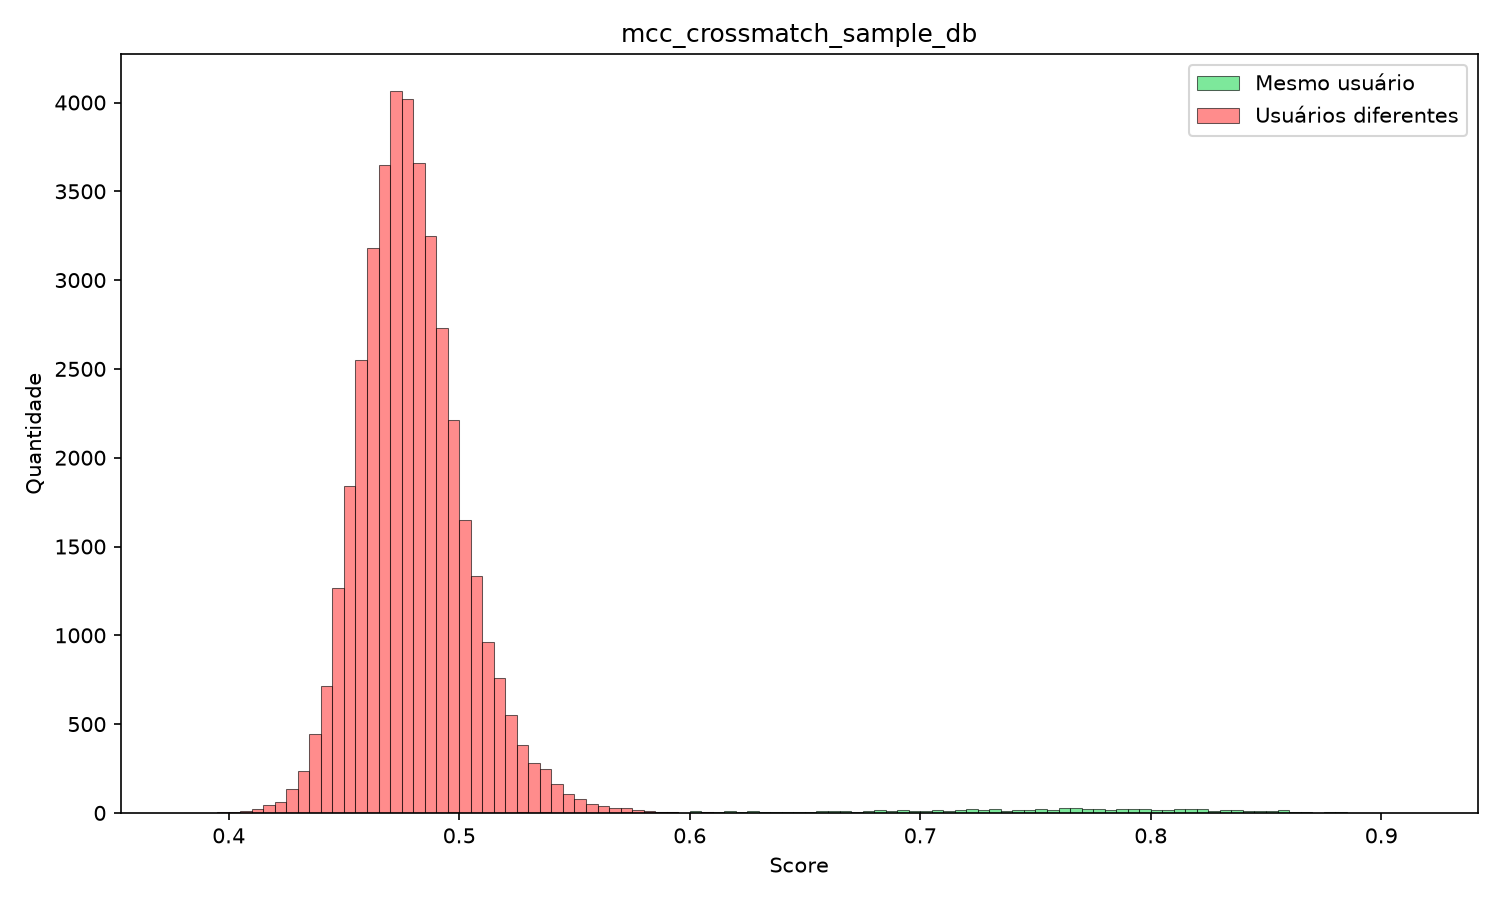
\includegraphics[width=0.32\textwidth]{figures/histograms/mcc_crossmatch_sample_db.png}}

\subfloat[DeepPrint - U.are.U]{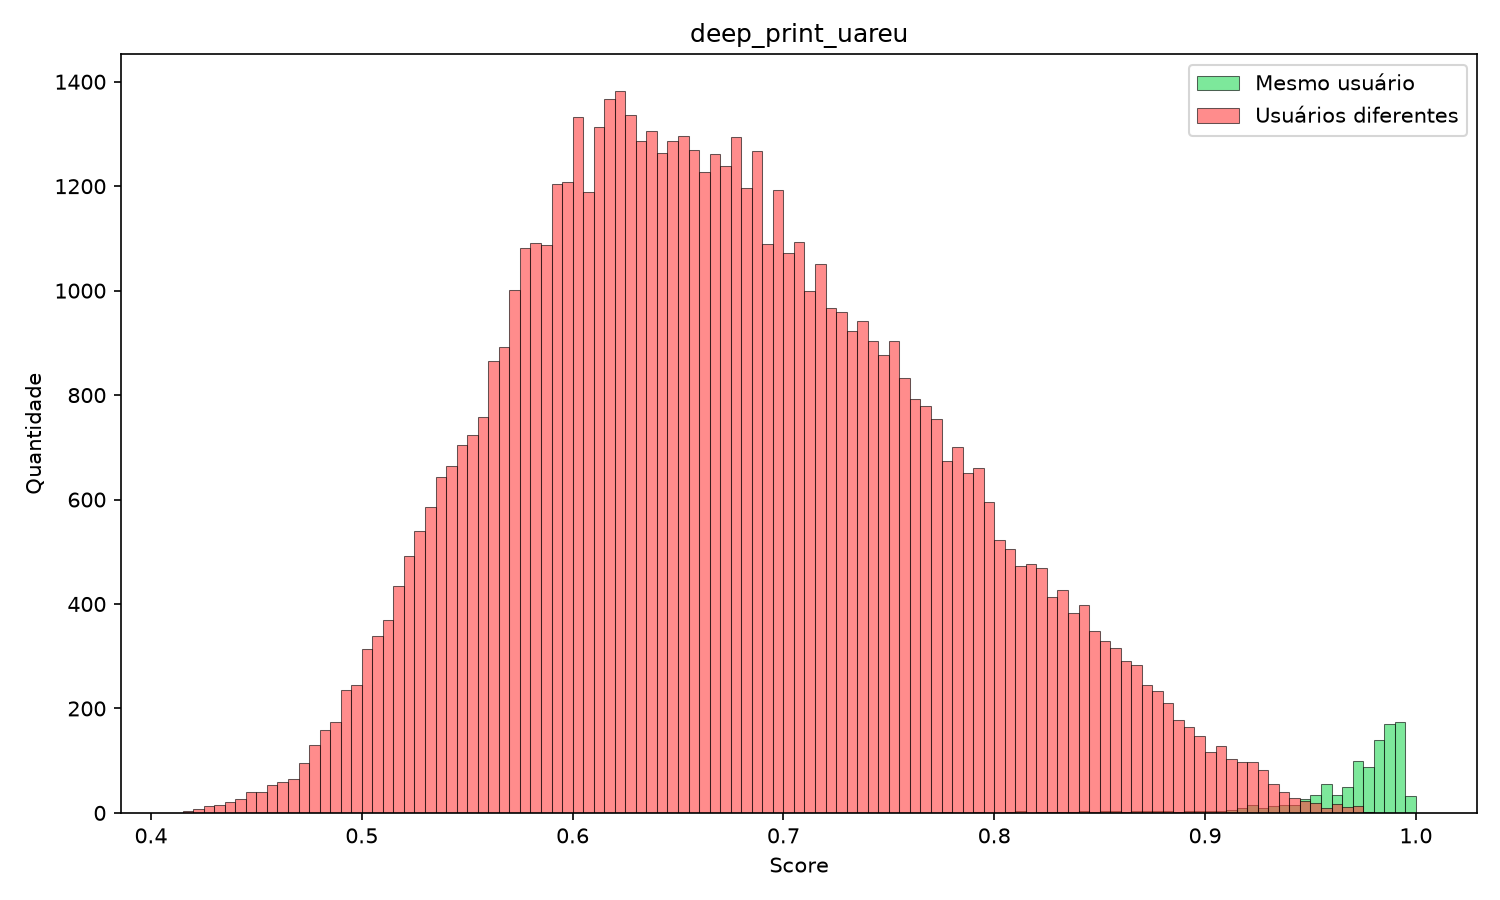
\includegraphics[width=0.32\textwidth]{figures/histograms/deep_print_uareu.png}}
\hfill
\subfloat[FLARE (Votação) - U.are.U]{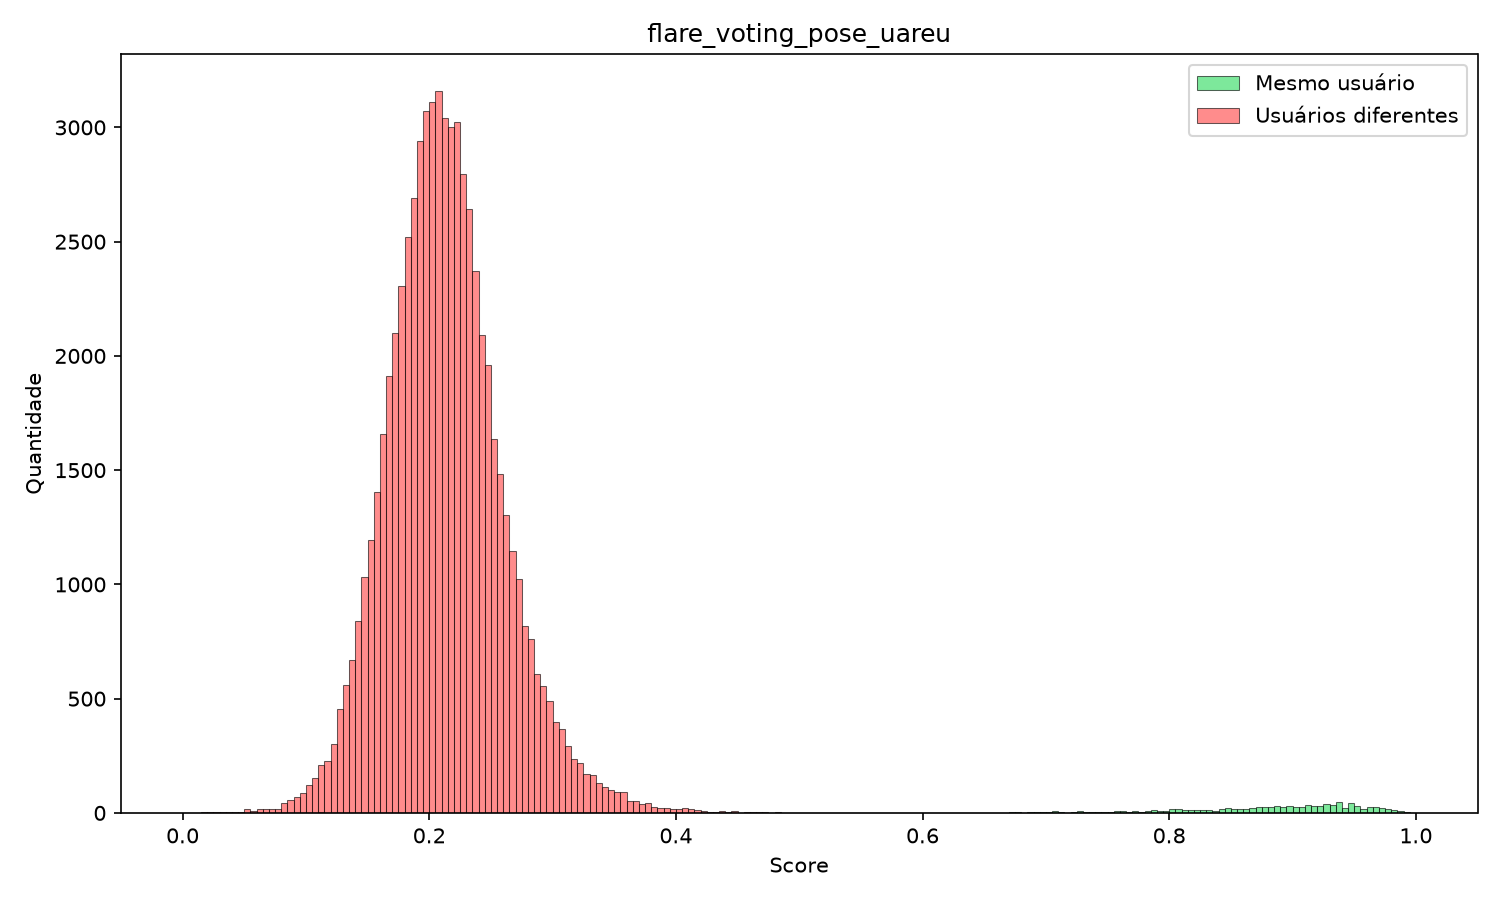
\includegraphics[width=0.32\textwidth]{figures/histograms/flare_voting_pose_uareu.png}}
\hfill
\subfloat[MCC - U.are.U]{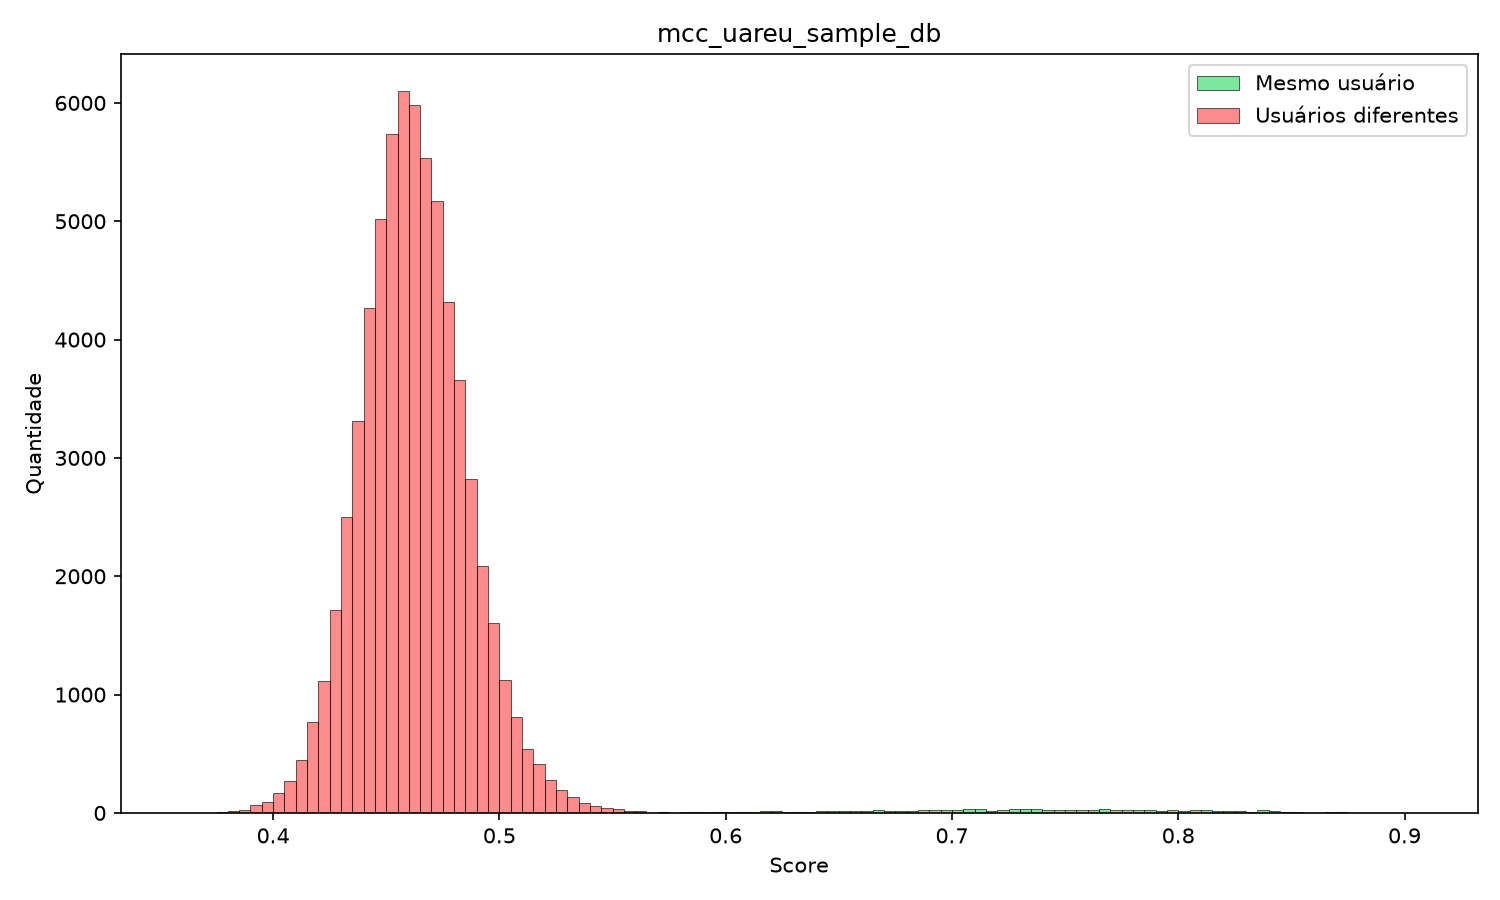
\includegraphics[width=0.32\textwidth]{figures/histograms/mcc_uareu_sample_db.png}}

\caption{Comparação da distribuição das pontuações de similaridade entre DeepPrint, FLARE com alinhamento por votação e MCC para os conjuntos CrossMatch e U.are.U da Neurotechnology.}\label{fig:histograms_neurotechnology}
\end{figure}


